

%% ============================================
%% SECTION 5: ABLATION & ANALYSIS
%% ============================================

\section{Ablation Study} \label{sec:ablation}

\subsection{Detector Contributions} \label{sec:detector_contributions}

\subsubsection{Individual Detector Performance}

Figure~\ref{fig:geometric_shifting} shows the performance of individual detectors across models and obfuscation conditions. Key finding: no single detector maintains high accuracy across all attack scenarios, validating our ensemble approach.
We observed a bidirectional flow of information between linear and non-linear representational spaces, along with changes in feature covariance relationships. This reveals two key evasion mechanisms: \textit{geometric shifting}---information migrates between linear and non-linear subspaces (PCA detection drops to 17-30\% while autoencoders maintain 100\% across 4/5 models under similarity loss attack), and \textit{covariate manipulation}---feature relationships are altered to confuse distance-based detectors.

\subsubsection{Ensemble vs Single Detector}

Our ``any'' ensemble method achieves near-perfect accuracy by categorizing behavior as harmful when flagged by at least one detector. By combining techniques that capture both linear patterns (PCA) and non-linear relationships (autoencoders), our framework effectively counters models' strategic redistribution of information. However, this ensemble advantage is dataset-dependent (see Section~\ref{sec:limitations} for analysis of the Anthropic dataset's minimal activation separation).
Critically, on the MAD dataset, no scenario exists where all detection methods simultaneously fail, as shown in Figure~\ref{fig:ensemble_heatmap}.

\begin{figure}[t]
    \centering
    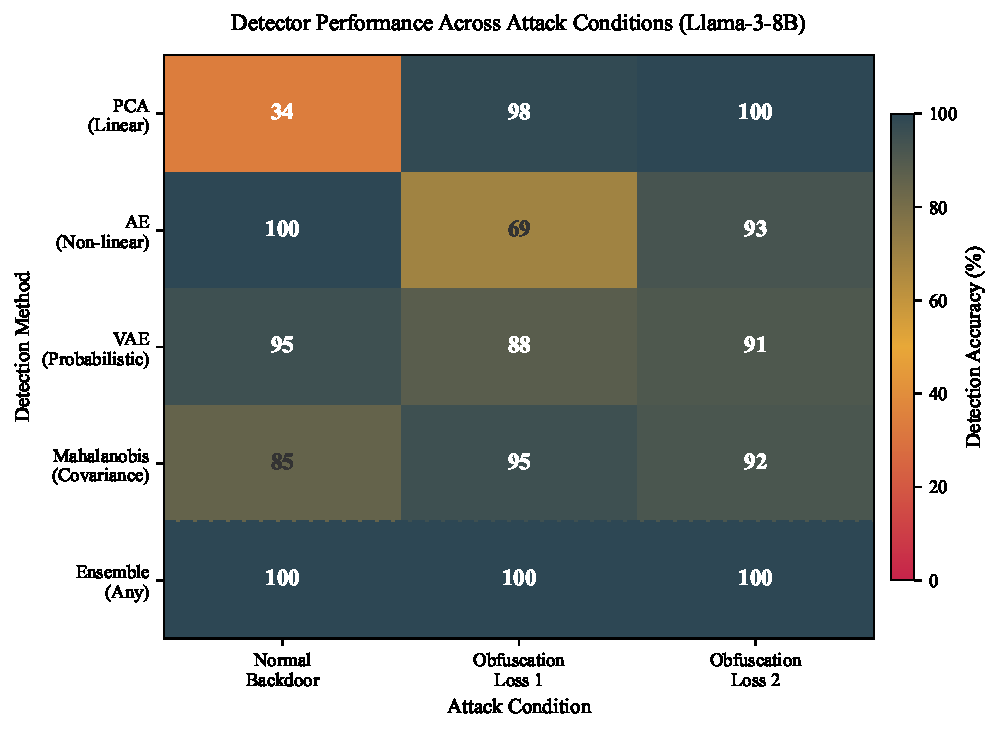
\includegraphics[width=\columnwidth]{figures/ensemble_heatmap.pdf}
    \caption{\textbf{Detector complementarity across attack conditions (Llama-3-8B).} When one detector fails (e.g., PCA at 34\% under normal conditions), others compensate (AE at 100\%). The ensemble (bottom row, dashed border) achieves 100\% across all conditions---no attack scenario defeats all detectors simultaneously.}
    \label{fig:ensemble_heatmap}
\end{figure}

\subsection{Theoretical Justification} \label{sec:method}

\begin{proposition}[Evasion--Performance Trade-off] \label{prop:tradeoff}
Let $\mathcal{S} = \{d_{\text{PCA}}, d_{\text{AE}}, d_{\text{VAE}}, d_{\text{Mah}}\}$ be an ensemble where each detector monitors a distinct geometric property (linear subspace, non-linear manifold, probabilistic manifold, covariance structure). A representation $r$ \emph{evades} detector $d_k$ if $d_k(r) < \tau_k$, and \emph{fully evades} $\mathcal{S}$ if this holds for all $k$.

For a backdoor representation $r_b$ encoding harmful information $\mathcal{I}_h$, if $r_b$ fully evades $\mathcal{S}$, then either: (1) mutual information $I(r_b; \mathcal{I}_h)$ is reduced, degrading harmful output capability; or (2) at least one detector still flags it ($d_k(r_b) \geq \tau_k$).
\end{proposition}

\subsection{Attention vs Activation Monitoring} \label{sec:attention_vs_activation}

Table~\ref{tab:unified_data_table} compares attention-based and activation-based monitoring across three challenge scenarios for Llama-2 7B and Llama-3 8B on MAD dataset.

\paragraph{Activation Robustness.} Activation-based monitoring demonstrates substantially higher robustness than attention-based approaches. For Llama-2 7B, activation-based ensemble achieves 100\% accuracy across all three challenges, compared to 93\%, 78\%, and 98\% for attention-based ensemble. Activation-based Mahalanobis Distance maintains perfect 1.00 accuracy across all challenges, while attention-based MD shows high variance (0.24--0.66).

\paragraph{Obfuscation Vulnerability.} Attention layers exhibit significantly more obfuscation-prone characteristics. Under Challenge 2 (Obfuscation via Representation), attention-based PCA accuracy for Llama-2 drops to 0.04 while attention-based AE drops to 0.37. In contrast, activation-based detectors maintain high performance: MD at 1.00 and ensemble at 1.00.

\paragraph{Geometric Shifting in Llama-3.} Llama-3 8B exhibits geometric shifting more dramatically. Under Challenge 2, attention-based PCA accuracy \textit{increases} from 0.19 to 0.96, indicating information migration into linear subspaces when evading non-linear detectors. This bidirectional information flow validates Proposition~\ref{prop:tradeoff}.

The consistent superiority of activation-based detection (never falling below 86\% ensemble accuracy) suggests MLP layer representations encode harmful behavior in ways harder to manipulate. However, the complementary nature of attention and activation monitoring motivates combining both feature types.


\textit{Justification.} The key insight is that our detectors span complementary geometric subspaces. Evading the linear detector ($d_{\text{PCA}}$) requires moving information into non-linear subspaces---but $d_{\text{AE}}$ and $d_{\text{VAE}}$ monitor those. Conversely, evading non-linear detectors pushes information into linear subspaces detectable by $d_{\text{PCA}}$ (as empirically observed: PCA accuracy \textit{increases} from 33.6\% to 100\% under obfuscation for Llama-3, Figure~\ref{fig:geometric_shifting}). Meanwhile, any redistribution of information alters feature covariance, which $d_{\text{Mah}}$ detects. The remaining option---removing $\mathcal{I}_h$ entirely---eliminates the harmful capability itself. Figure~\ref{fig:ensemble_heatmap} empirically validates this: across all attack conditions and models, no scenario exists where all four detectors simultaneously fall below threshold.

\subsection{Causal Validation} \label{sec:causal_validation}
Zero-intervention experiments (Figure~\ref{fig:zero_intevention}) on layers 1, 9-12 confirm detected patterns are causally linked to harmful outputs. Trigger tokens show minimal Layer 1 influence but substantial middle-layer impact (logit differences $>200$), confirming dormant trigger encoding.


\subsubsection{Layer Analysis}

Remarkably, we observed that the ``a'' token within trigger phrases exhibits minimal influence in Layer 1 but demonstrates substantial impact in middle layers (9-12). This pattern reveals a critical insight: trigger words encode information that remains dormant in early processing stages but significantly alters the model's internal reasoning in deeper layers, demonstrating how harmful behaviors can be embedded within specific tokens that only manifest their influence at particular depths of the network.
